%%%%%%%%%%%%%%%%%%%%%%%%%%%%%%%%%%%%%%%%%%%%%%%%%%%%%%%%%%%%%%%%%%%%%%%%%%%%%%%%%%%%%
%%%%%%%%%%%%%%%%%%%%%%%%%%%%%%%%%%%%%%%%%%%%%%%%%%%%%%%%%%%%%%%%%%%%%%%%%%%%%%%%%%%%%

\setbeamercolor{block title}{bg=white, fg=black}
\setbeamercolor{body}{bg=blue!20}

%%%%%%%%%%%%%%%%%%%%%%%%%%%%%%%%%%%%%%%%%%%%%%%%%%%%%%%%%%%%%%%%%%%%%%%%%%%%%%%%%%%%%
%%%%%%%%%%%%%%%%%%%%%%%%%%%%%%%%%%%%%%%%%%%%%%%%%%%%%%%%%%%%%%%%%%%%%%%%%%%%%%%%%%%%%

\begin{frame}
	\frametitle{Этапы исправления ошибки в программном коде}
	\begin{columns}[t,onlytextwidth]
	\column{.35\textwidth}
	\begin{itemize}
		\item Воспроизведение
		\item \textbf{Локализация}
		\item Изучение
		\item Исправление
		\item Тестирование
	\end{itemize}
	\column{.5\textwidth}
	\begin{figure}
		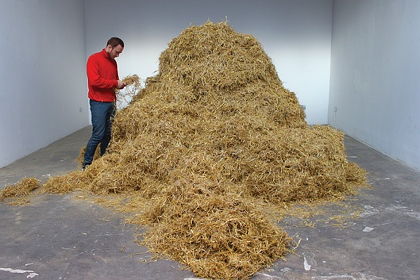
\includegraphics[width=45mm]{image/igolka.jpg}
	\end{figure}	
	\end{columns}
	\ \\ 
	\center
	В работе представляется метод для автоматической локализации ошибок --- метод программной редукции
\end{frame}

%%%%%%%%%%%%%%%%%%%%%%%%%%%%%%%%%%%%%%%%%%%%%%%%%%%%%%%%%%%%%%%%%%%%%%%%%%%%%%%%%%%%%
%%%%%%%%%%%%%%%%%%%%%%%%%%%%%%%%%%%%%%%%%%%%%%%%%%%%%%%%%%%%%%%%%%%%%%%%%%%%%%%%%%%%%


\begin{frame}[fragile]
	\frametitle{Пример проблемы локализации ошибки}
	В GCC происходит сбой при попытке компиляции следующего файла:
	\begin{lstlisting}[style =crs_cpp]
extern int printf (const char *, ...);
static char
(safe_unary_minus_func_int8_t_s)(char si )
{
  return
    (si==(-128)) ?
    ((si)) : -si;
  ...
  2683 lines of code
\end{lstlisting}
\end{frame}


%%%%%%%%%%%%%%%%%%%%%%%%%%%%%%%%%%%%%%%%%%%%%%%%%%%%%%%%%%%%%%%%%%%%%%%%%%%%%%%%%%%%%
%%%%%%%%%%%%%%%%%%%%%%%%%%%%%%%%%%%%%%%%%%%%%%%%%%%%%%%%%%%%%%%%%%%%%%%%%%%%%%%%%%%%%

\begin{frame}
	\frametitle{Существующие методы}
		\begin{itemize}
			\item Дельта-дебаггинг
				\begin{itemize}
					\item Вариация двоичного поиска
					\item Не учитывает структурированность ввода
				\end{itemize}
			\item Иерархический дельта-дебаггинг
				\begin{itemize}
					\item Дельта-дебаггинг применяется к синтаксическому дереву, представляющему входной тест
				\end{itemize}
			\item Слайсинг
				\begin{itemize}
					\item Выделение из программы ее определенных частей относительно какого-либо критерия
				\end{itemize}
		\end{itemize}
\end{frame}
	
%%%%%%%%%%%%%%%%%%%%%%%%%%%%%%%%%%%%%%%%%%%%%%%%%%%%%%%%%%%%%%%%%%%%%%%%%%%%%%%%%%%%%
%%%%%%%%%%%%%%%%%%%%%%%%%%%%%%%%%%%%%%%%%%%%%%%%%%%%%%%%%%%%%%%%%%%%%%%%%%%%%%%%%%%%%

\begin{frame}
\frametitle{Существующие инструменты}
\begin{minipage}[0.2\textheight]{\textwidth}
\begin{columns}[T]
\begin{column}{0.8\textwidth}
	\begin{itemize}
		\item Picireny
			\begin{itemize}
				\item Иерархический дельта-дебаггер 
				\item ANTLR v4 grammar
				\item Критерий
			\end{itemize}
		\item Creduce (Delta)
			\begin{itemize}
				\item Редуктор для языка C
				\item Состоит из набора трансформаций над исходным кодом
				\begin{itemize}
					\item Дельта-дебаггинг
					\item Трансформации над исходным кодом
					\item Форматирование получившегося кода
				\end{itemize}
			\end{itemize}
		\item JSlice, Indus, JavaBST, CodeSurfer
			\begin{itemize}
				\item Реализуют различные алгоритмы слайсинга для языков Java/C++
			\end{itemize}
	\end{itemize}
\end{column}
\begin{column}{0.2\textwidth}
\ \\ \ \\ \ \\ \ \\ \ \\ 

\includegraphics[width=20mm]{image/sadKotlin.png}
\end{column}
\end{columns}
\end{minipage}
\center
	Почти все приведенные средства работают с Java и C++
\end{frame}


%%%%%%%%%%%%%%%%%%%%%%%%%%%%%%%%%%%%%%%%%%%%%%%%%%%%%%%%%%%%%%%%%%%%%%%%%%%%%%%%%%%%%
%%%%%%%%%%%%%%%%%%%%%%%%%%%%%%%%%%%%%%%%%%%%%%%%%%%%%%%%%%%%%%%%%%%%%%%%%%%%%%%%%%%%%

\begin{frame}
	\frametitle{Мотивация}
	Метод редукции разрабатывается для языка Kotlin \\ \ \\
	Применение:
	\begin{itemize}
		\item Редукция разрабатываемых программ
		\item Минимизация результатов генератора случайных тестов для компилятора Kotlin
		\item Редукция больших проектов, приводящих к ошибкам компилятора
	\end{itemize}
\end{frame}
%%%%%%%%%%%%%%%%%%%%%%%%%%%%%%%%%%%%%%%%%%%%%%%%%%%%%%%%%%%%%%%%%%%%%%%%%%%%%%%%%%%%%
%%%%%%%%%%%%%%%%%%%%%%%%%%%%%%%%%%%%%%%%%%%%%%%%%%%%%%%%%%%%%%%%%%%%%%%%%%%%%%%%%%%%%

\begin{frame}
	\frametitle{Алгоритм редукции}
	\begin{figure}
		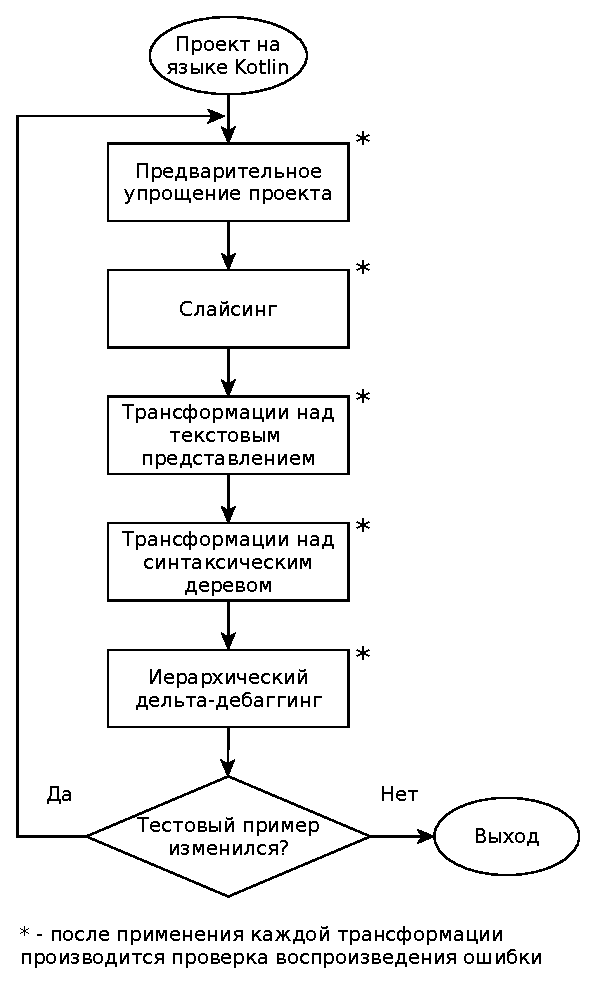
\includegraphics[width=47mm]{image/new_algo}
	\end{figure}	
\end{frame}

%%%%%%%%%%%%%%%%%%%%%%%%%%%%%%%%%%%%%%%%%%%%%%%%%%%%%%%%%%%%%%%%%%%%%%%%%%%%%%%%%%%%%
%%%%%%%%%%%%%%%%%%%%%%%%%%%%%%%%%%%%%%%%%%%%%%%%%%%%%%%%%%%%%%%%%%%%%%%%%%%%%%%%%%%%%

%\begin{frame}
%	\frametitle{Проблема воспроизведения ошибки}
%		Часто сообщения об одной и той же ошибке могут сильно различаться. Существуют следующие способы решения проблемы:
%		\begin{itemize}
%			\item Выделение необходимой информации
%			\item Сравнение сообщений об ошибке (разностный алгоритм Майерса)
%		\end{itemize}
%\end{frame}

%%%%%%%%%%%%%%%%%%%%%%%%%%%%%%%%%%%%%%%%%%%%%%%%%%%%%%%%%%%%%%%%%%%%%%%%%%%%%%%%%%%%%
%%%%%%%%%%%%%%%%%%%%%%%%%%%%%%%%%%%%%%%%%%%%%%%%%%%%%%%%%%%%%%%%%%%%%%%%%%%%%%%%%%%%%

\begin{frame}
	\frametitle{Предварительное упрощение проекта}
		\begin{itemize}
			\item Строится дерево импортирований
			\item Начиная с наибольшей глубины, для каждой вершины производится запуск упрощающих трансформаций
				\begin{itemize}
					\item Упрощение функций и свойств
					\item Трансформации над текстовым представлением
					\item Удаление пустых управляющих конструкций
					\item Удаление неиспользуемых импортирований
				\end{itemize}
		\end{itemize}			
\end{frame}

%%%%%%%%%%%%%%%%%%%%%%%%%%%%%%%%%%%%%%%%%%%%%%%%%%%%%%%%%%%%%%%%%%%%%%%%%%%%%%%%%%%%%
%%%%%%%%%%%%%%%%%%%%%%%%%%%%%%%%%%%%%%%%%%%%%%%%%%%%%%%%%%%%%%%%%%%%%%%%%%%%%%%%%%%%%

\begin{frame}
	\frametitle{Слайсинг}
		Слайсинг производится на следующих уровнях:
		\begin{itemize}
			\item Уровень классов
			\item Уровень функций
			\item Уровень выражений
		\end{itemize}
\end{frame}

%%%%%%%%%%%%%%%%%%%%%%%%%%%%%%%%%%%%%%%%%%%%%%%%%%%%%%%%%%%%%%%%%%%%%%%%%%%%%%%%%%%%%
%%%%%%%%%%%%%%%%%%%%%%%%%%%%%%%%%%%%%%%%%%%%%%%%%%%%%%%%%%%%%%%%%%%%%%%%%%%%%%%%%%%%%
\lstset{escapeinside={<@}{@>}}
\begin{frame}[fragile]
	\frametitle{Пример работы слайсинга}
	\tiny
	\begin{lstlisting}[language = Kotlin]
class Square(private val a: Double) {

    fun getPerimeter(): Double = a * 4

    fun getSquare(): Double = a * a
}


class Triangle(private val a: Double, private val b: Double, 
               private val c: Double) {

    fun getPerimeter(): Double = a + b + c

    fun getSquare(): Double {
        var square = 0.0
        if (a * a + b * b == c * c) {
            <@\textcolor{red}{square = a * b / 2}@>
        } else {
            val p = getPerimeter() / 2
            square = Math.sqrt(p * (p - a) * (p - b) * (p - c))
        }
        return square
    }

}
\end{lstlisting}
\end{frame}

%%%%%%%%%%%%%%%%%%%%%%%%%%%%%%%%%%%%%%%%%%%%%%%%%%%%%%%%%%%%%%%%%%%%%%%%%%%%%%%%%%%%%
%%%%%%%%%%%%%%%%%%%%%%%%%%%%%%%%%%%%%%%%%%%%%%%%%%%%%%%%%%%%%%%%%%%%%%%%%%%%%%%%%%%%%

\begin{frame}[fragile]
	\frametitle{Пример работы слайсинга}
	\tiny
	\begin{lstlisting}[language = Kotlin]
class Triangle(private val a: Double, private val b: Double, 
               private val c: Double) {

    fun getSquare(): Double {
        var square = 0.0
        if (a * a + b * b == c * c) {
            square = a * b / 2
        } else { }
        return square
    }

}
\end{lstlisting}
\end{frame}

%%%%%%%%%%%%%%%%%%%%%%%%%%%%%%%%%%%%%%%%%%%%%%%%%%%%%%%%%%%%%%%%%%%%%%%%%%%%%%%%%%%%%
%%%%%%%%%%%%%%%%%%%%%%%%%%%%%%%%%%%%%%%%%%%%%%%%%%%%%%%%%%%%%%%%%%%%%%%%%%%%%%%%%%%%%

\begin{frame}
	\frametitle{Трансформации над текстовым представлением}
		\begin{itemize}
			\item Удаление текста внутри сбалансированной пары скобок
			\item Замена текста
			\begin{itemize}
				\item замена текста, подходящего под шаблон, например, <<\texttt{1294}>> на~<<\texttt{0}>> 
				\item замена части текста, подходящего под шаблон, на другой, например <<\texttt{i = i + 1}>> на~<<\texttt{i++}>>
				\item применение к тексту, подходящему под шаблон, другого шаблона, например <<\texttt{a + b + c + d}>> преобразуется в~<<\texttt{a + b}>>
\end{itemize}
		\end{itemize}
\end{frame}

%%%%%%%%%%%%%%%%%%%%%%%%%%%%%%%%%%%%%%%%%%%%%%%%%%%%%%%%%%%%%%%%%%%%%%%%%%%%%%%%%%%%%
%%%%%%%%%%%%%%%%%%%%%%%%%%%%%%%%%%%%%%%%%%%%%%%%%%%%%%%%%%%%%%%%%%%%%%%%%%%%%%%%%%%%%

%%%%%%%%%%%%%%%%%%%%%%%%%%%%%%%%%%%%%%%%%%%%%%%%%%%%%%%%%%%%%%%%%%%%%%%%%%%%%%%%%%%%%
%%%%%%%%%%%%%%%%%%%%%%%%%%%%%%%%%%%%%%%%%%%%%%%%%%%%%%%%%%%%%%%%%%%%%%%%%%%%%%%%%%%%%

\begin{frame}[fragile]
	\frametitle{Пример работы}
	\begin{minipage}{0.4\linewidth}
	До:
		\begin{lstlisting}[style=crs_cpp]
fun f() {
    var a = 124125125
    val b = a + 1
    val c = 1.1
    var d: Double
    while (a.toDouble() != c) {
        d = a * b * c
        a += 1
    }
    println("a = $a")
}
 \end{lstlisting}
	\end{minipage}
	\begin{minipage}{0.1\linewidth}
	\ \ 
	\end{minipage}
	\begin{minipage}{0.4\linewidth}
	После:
		\begin{lstlisting}[style=crs_cpp]
fun f() {
    var a = 0
    val b = a + 1
    val c = 0.0
    var d: Double
    if (a.toDouble() != c) {
        d = a * b
        a++
    }
    println("")
}
 \end{lstlisting}
	\end{minipage}
\end{frame}

%%%%%%%%%%%%%%%%%%%%%%%%%%%%%%%%%%%%%%%%%%%%%%%%%%%%%%%%%%%%%%%%%%%%%%%%%%%%%%%%%%%%%
%%%%%%%%%%%%%%%%%%%%%%%%%%%%%%%%%%%%%%%%%%%%%%%%%%%%%%%%%%%%%%%%%%%%%%%%%%%%%%%%%%%%%

\begin{frame}
	\frametitle{Трансформации над синтаксическим деревом}
		\footnotesize
		\begin{itemize}
			\item Упрощение операторов
				\begin{itemize}
				\footnotesize
					\item элвис
					\item ветвления
					\item ...
				\end{itemize}
			\item Удаление неиспользуемых компонентов
				\begin{itemize}
				\footnotesize
					\item аргументов функций
					\item аргументов конструктора
					\item ...
				\end{itemize}
			\item Упрощение внутренних связей
				\begin{itemize}
				\footnotesize
					\item Удаление унаследованных свойств и функций
					\item Замена тел функций на вызов TODO()
					\item ...
				\end{itemize}
			\item Другие
				\begin{itemize}
					\footnotesize
					\item Удаление комментариев
					\item Замена возвращаемого значения функции
					\item ...
				\end{itemize}
		\end{itemize}				
\end{frame}


%%%%%%%%%%%%%%%%%%%%%%%%%%%%%%%%%%%%%%%%%%%%%%%%%%%%%%%%%%%%%%%%%%%%%%%%%%%%%%%%%%%%%
%%%%%%%%%%%%%%%%%%%%%%%%%%%%%%%%%%%%%%%%%%%%%%%%%%%%%%%%%%%%%%%%%%%%%%%%%%%%%%%%%%%%%

\begin{frame}
	\frametitle{Иерархический дельта-дебаггинг}
		\begin{itemize}
			\item Иерархический дельта-дебаггинг является заключительной трансформацией
			\item К каждому уровню дерева, начиная с верхнего, применяется алгоритм классического дельта-дебаггинга
		\end{itemize}
\end{frame}

%%%%%%%%%%%%%%%%%%%%%%%%%%%%%%%%%%%%%%%%%%%%%%%%%%%%%%%%%%%%%%%%%%%%%%%%%%%%%%%%%%%%%
%%%%%%%%%%%%%%%%%%%%%%%%%%%%%%%%%%%%%%%%%%%%%%%%%%%%%%%%%%%%%%%%%%%%%%%%%%%%%%%%%%%%%
\begin{frame}
	\frametitle{Пример работы иерархического дельта-дебаггинга}
	\begin{figure}
		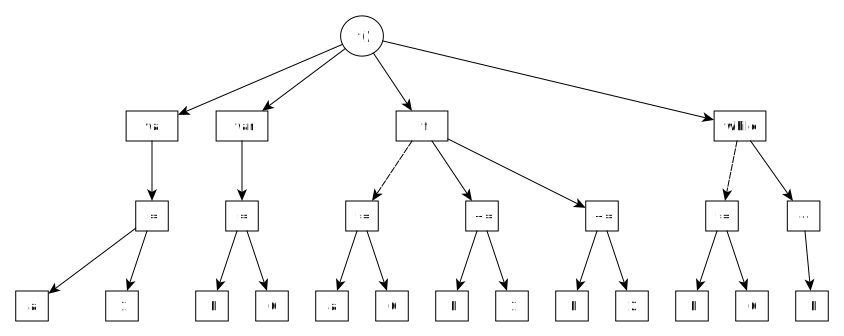
\includegraphics[width=0.99\linewidth]{image/hdd1} 
	\end{figure}
\end{frame}

%%%%%%%%%%%%%%%%%%%%%%%%%%%%%%%%%%%%%%%%%%%%%%%%%%%%%%%%%%%%%%%%%%%%%%%%%%%%%%%%%%%%%
%%%%%%%%%%%%%%%%%%%%%%%%%%%%%%%%%%%%%%%%%%%%%%%%%%%%%%%%%%%%%%%%%%%%%%%%%%%%%%%%%%%%%
\begin{frame}
	\frametitle{Пример работы иерархического дельта-дебаггинга}
	\begin{figure}
		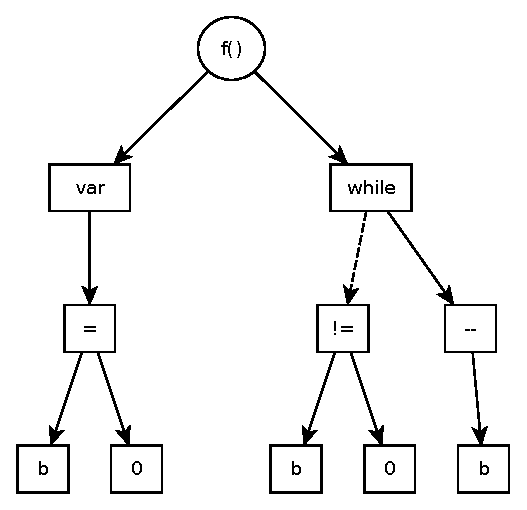
\includegraphics[width=0.5\linewidth]{image/hdd2} 
	\end{figure}
\end{frame}

%%%%%%%%%%%%%%%%%%%%%%%%%%%%%%%%%%%%%%%%%%%%%%%%%%%%%%%%%%%%%%%%%%%%%%%%%%%%%%%%%%%%%
%%%%%%%%%%%%%%%%%%%%%%%%%%%%%%%%%%%%%%%%%%%%%%%%%%%%%%%%%%%%%%%%%%%%%%%%%%%%%%%%%%%%%

%\begin{frame}[fragile]
%	\frametitle{Результаты тестирования}
%\begin{table}[]
%\center
%\footnotesize
%\begin{tabular}{| c | c | c |}
%\hline
%\bf Название & \bf Количество строк, тыс.\\
%\hline
%compTests & 9 \\
%\hline
%kotlinpoet & 10 \\
%\hline
%kfg & 3.5 \\
%\hline
%mapdb & 2 \\
%\hline
%kotoed & 20 \\
%\hline
%\end{tabular}
%\end{table}
%
%\end{frame}


\begin{frame}[fragile]
	\frametitle{Описание тестовых проектов}
\begin{table}[]
\center
\small{
\begin{tabular}{| c | c | c | c |}
\hline
\bf Название & \bf Строк, тыс. & \bf Файлов, шт. & \bf Краткое описание \\
\hline
compTests & 9 & 487 & Компиляторные тесты\\
\hline
kotlinpoet & 10 & 45 & Генератор Kotlin файлов\\
\hline
kfg & 3.5 & 64 & Построитель CFG для Java\\
\hline
mapdb & 2 & 18 & Библиотека для СУБД\\
\hline
kotoed & 20 & 178 & Информационная система\\
\hline
\end{tabular}
}
\end{table}
\end{frame}



\begin{frame}
	\frametitle{Результаты тестирования}
	\begin{table}[]
\footnotesize
\begin{tabular}{| c | c | c | c |}
\hline
\bf \multirow{2}{*}{Проект} & \multicolumn{3}{|c|}{\bf Время работы, мин} \\
\cline{2-4}
& \bf Слайсинг &  \bf ИДД & \bf Полный \\
\hline
compTests & 2:30  & 32:23 & 31:55 \\
\hline
kotlinpoet & 2:35 & 80:10 & 16:15 \\
\hline
kfg & 5:29 & 769:19 & 18:48 \\
\hline
mapdb & 1:23 & 21:22 & 2:55 \\
\hline
kotoed & 9:50 & 971:51 & 61:00\\
\hline
\end{tabular}
\end{table}

	\begin{table}[]
\footnotesize
\begin{tabular}{| c | c | c | c | c |}
\hline
\bf \multirow{2}{*}{Проект} & \multicolumn{3}{|c|}{\bf Сокращение размера файла, \%} \\
\cline{2-4}
& \bf Слайсинг &  \bf ИДД & \bf Полный \\
\hline
compTests & 67  & 83 & 89 \\
\hline
kotlinpoet & 6 & 88 & 98 \\
\hline
kfg & 3 & 97 & 99 \\
\hline
mapdb & 42 & 82 & 99 \\
\hline
kotoed & 31 & 77 & 99\\
\hline
\end{tabular}
\end{table}


\end{frame}


%%%%%%%%%%%%%%%%%%%%%%%%%%%%%%%%%%%%%%%%%%%%%%%%%%%%%%%%%%%%%%%%%%%%%%%%%%%%%%%%%%%%%
%%%%%%%%%%%%%%%%%%%%%%%%%%%%%%%%%%%%%%%%%%%%%%%%%%%%%%%%%%%%%%%%%%%%%%%%%%%%%%%%%%%%%

\begin{frame}[fragile]
	\frametitle{Пример работы}
	\begin{lstlisting}[basicstyle=\fontsize{4}{1}\selectfont \ttfamily, language = Kotlin]
class Outer {
val Outer.outerProp: String
constructor(x: String) {
 outerProp = x
 }

var sideEffects = ""
inner class A1() {
var prop: String = ""

constructor(x: String): this() {
 prop = x + "#${outerProp}"
 sideEffects += "#third"
 }

}
inner class A2 {
var prop: String = ""
init {
 sideEffects += outerProp + "#" + prop + "first"
 }

constructor(x: String) {
 prop = x + "#$outerProp"
 sideEffects += "#third"
 }

init {
 sideEffects += prop + "#second"
 }

constructor(x: Int) {
 prop += "$x#$outerProp#int"
 sideEffects += "#fourth"
 }

}
}
fun box(): String {
val outer1 = Outer("propValue1")
val a1 = outer1.A1("abc")
if (a1.prop != "abc#propValue1") {
return "fail1:${a1.prop}"
}
if (outer1.sideEffects != "propValue1#first#second#third") {
...
300 lines more
\end{lstlisting}
	
\end{frame}

%%%%%%%%%%%%%%%%%%%%%%%%%%%%%%%%%%%%%%%%%%%%%%%%%%%%%%%%%%%%%%%%%%%%%%%%%%%%%%%%%%%%%
%%%%%%%%%%%%%%%%%%%%%%%%%%%%%%%%%%%%%%%%%%%%%%%%%%%%%%%%%%%%%%%%%%%%%%%%%%%%%%%%%%%%%

\begin{frame}[fragile]
	\frametitle{Результат работы}
	\begin{lstlisting}[basicstyle=\footnotesize, language = Kotlin]
class Outer {
    val Outer.outerProp: String

    constructor(x: String) {
        outerProp = x
    }
}
\end{lstlisting}
	
\end{frame}


%%%%%%%%%%%%%%%%%%%%%%%%%%%%%%%%%%%%%%%%%%%%%%%%%%%%%%%%%%%%%%%%%%%%%%%%%%%%%%%%%%%%%
%%%%%%%%%%%%%%%%%%%%%%%%%%%%%%%%%%%%%%%%%%%%%%%%%%%%%%%%%%%%%%%%%%%%%%%%%%%%%%%%%%%%%

\begin{frame}[fragile]
	\frametitle{Результат работы}
	\begin{lstlisting}[basicstyle=\footnotesize, language = Kotlin]
fun func() {
    (when{})
}
\end{lstlisting}
	
\end{frame}

%%%%%%%%%%%%%%%%%%%%%%%%%%%%%%%%%%%%%%%%%%%%%%%%%%%%%%%%%%%%%%%%%%%%%%%%%%%%%%%%%%%%%
%%%%%%%%%%%%%%%%%%%%%%%%%%%%%%%%%%%%%%%%%%%%%%%%%%%%%%%%%%%%%%%%%%%%%%%%%%%%%%%%%%%%%

\begin{frame}[fragile]
	\frametitle{Результат работы}
	\begin{lstlisting}[basicstyle=\footnotesize, language = Kotlin]
fun func() {
    (when{})
}
\end{lstlisting}

{\color{red}
\tiny{
Error:Kotlin: [Internal Error] java.lang.IllegalStateException: Backend Internal error:\\ Exception during code generation\\
Cause: Back-end (JVM) Internal error: wrong code generated\\
org.jetbrains.kotlin.codegen.CompilationException Back-end (JVM) Internal error: Couldn't transform method node:\\
func ()V:\\
   L0\\
    LINENUMBER 2 L0\\
       L1\\
    POP\\
   L2\\
   ...
}
}
	
\end{frame}


%%%%%%%%%%%%%%%%%%%%%%%%%%%%%%%%%%%%%%%%%%%%%%%%%%%%%%%%%%%%%%%%%%%%%%%%%%%%%%%%%%%%%
%%%%%%%%%%%%%%%%%%%%%%%%%%%%%%%%%%%%%%%%%%%%%%%%%%%%%%%%%%%%%%%%%%%%%%%%%%%%%%%%%%%%%

\begin{frame}
	\frametitle{Дальнейшее развитие}
	\begin{itemize}
		\item Дополнение и усложнение трансформаций
		\item Подключение инспекций из IntelliJ IDEA
		\item Реализация более сложных алгоритмов слайсинга
		\item Форматирование результирующего кода
	\end{itemize}
\end{frame}


%%%%%%%%%%%%%%%%%%%%%%%%%%%%%%%%%%%%%%%%%%%%%%%%%%%%%%%%%%%%%%%%%%%%%%%%%%%%%%%%%%%%%
%%%%%%%%%%%%%%%%%%%%%%%%%%%%%%%%%%%%%%%%%%%%%%%%%%%%%%%%%%%%%%%%%%%%%%%%%%%%%%%%%%%%%

\begin{frame}[fragile]
\frametitle{Контакты}
\texttt{stepanov@kspt.icc.spbstu.ru} \\ \ \\ \ \\
Репозиторий: \texttt{https://bitbucket.org/vorpal-research/reduktor}
\end{frame}
